This chapter provides an overview of \acp{MAS}, as a mean to engineer intelligent applications.
%
\acp{MAS} are a broad research area at the intersection between \ac{AI} and software engineering.
%
Autonomous agents are used as the main abstraction to model and implement complex software systems. The behavior of such agents can be either programmed, learned or, more recently, generated through the use of \ac{GenAI} techniques. 

In this thesis, we mainly consider programmed agents, as we are interested in using agents to encapsulate business logic that can automate processes and activities in the context of \ac{DT}-based systems. 
%
Accordingly, the chapter introduces the research area which follows under the broad umbrella of \ac{AOSE} and more specifically \ac{AOP} as a paradigm to engineer and program \acp{MAS}. 
%
We specifically focus on \ac{BDI} agents, as they are amongst the most widely adopted agent model for programmed agents, capable of encoding domain and procedural knowledge through the cognitive abstractions they provide, thus making \ac{BDI} agents excellent candidates for reliable and explainable intelligent applications. 

%=======================================================
\section{History and Definitions}
%=======================================================

In order to understand the concept of \acp{MAS}, it is important to first understand what an \emph{agent} is.
%
Despite the term being widely used in different contexts~\cite{wooldridge1995ker} with different interpretations, a commonly accepted definition is the following:

\begin{quote}
    An agent is a computer system that is situated in some environment,
    and that is capable of autonomous action in this environment in order
    to meet its design objectives~\cite{2009wooldridge}.
\end{quote}

The definition highlights the key characteristics of an agent. 
%
Namely, an agent is \emph{situated} in an environment which can be either physical (e.g., for a robotic system) or virtual (e.g., for a fully software agent).
%
The environment provides the agent with an external context that can be perceived, influencing the behavior of the agent, and affected by the agent actions to reach its objectives.
%
\Cref{fig:agent-environment} shows the relationship between an agent and its environment. The agent receives \emph{percepts} from the environment through its sensors, and performs actions upon the environment through its \emph{effectors}.
%
The agent is also \emph{autonomous}, meaning that it can operate without direct intervention from humans or other systems, and has control over its actions and internal state.
%
Finally, the agent is \emph{goal-oriented}, as it is designed to achieve specific objectives, which can be explicitly defined or learned over time.

\begin{figure}[t]
    \centering
    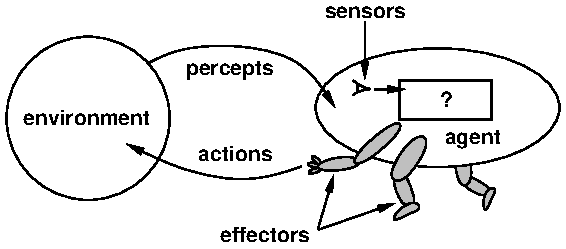
\includegraphics[width=0.8\textwidth]{figures/agent-environment-original.pdf}
    \caption{Classic schematic representation of an agent and its interaction with the environment, from \cite{1995russell-norvig}.}
    \label{fig:agent-environment}
\end{figure}

It is possible to distinguish between a \emph{weak} and \emph{strong} notion of agency~\cite{wooldridge1995ker}.
%
The weak notion of agency refers to systems that exhibit some characteristics of agents, namely autonomy, reactivity, pro-activeness, and social ability. 
%
This kind of agents are usually employed to model concurrent and distributed systems. 
%
The strong notion of agency, instead, derives from research on \ac{AI} and envisions agents as \emph{intelligent} entities, modeled using \emph{mentalistic} notions~\cite{Shoham_1993} to mimic human cognitive capabilities. 

The definitions of \emph{agent} focus on the properties of an agent and its behavior, leaving implementation details open. 
%
This has led to the development of different agent architectures to implement agents in software systems. 
%
The taxonomy of agent models proposed by Russell and Norvig~\cite{1995russell-norvig} distinguishes between increasingly complex agent models: 
\begin{description}
    \item[Simple Reflex Agents] operate on a set of predefined trigger-action rules and to respond to stimuli from the environment.
    \item[Model-Based Reflex Agents] keep an internal model of the environment, updating it over time, and allowing them to make decisions based on both current perceptions and past experiences.
    \item[Goal-Based Agents] are designed to achieve specific goals. They can evaluate different actions not only based on the model of the environment, but also on the potential of achieving their goal, allowing for more flexible and adaptive behavior.
    \item[Utility-Based Agents] not only aim to achieve goals but also consider the desirability of different outcomes. They use a utility function to evaluate the potential benefits of various actions, enabling them to make decisions that maximize overall satisfaction.
    \item[Learning Agents] can improve their performance over time through learning from experiences. They can adapt to changing environments and optimize their behavior based on feedback, making them more robust and effective in dynamic settings.
\end{description}

Implementing an agent essentially boils down to specify its behavior in response to its perceptions of the environment, with different degrees of complexity. 
%
How this is achieved depends on the agent architecture and model adopted, but we can generally  distinguish two main categories: \emph{programmed} or \emph{learning} agents, depending on whether their behavior is explicitly defined by a developer or learned from data and experience. 
%
Although the boundary between the two categories is not always clear-cut, as learning techniques can be used to complement programmed behavior~\cite{Bordini_El_Fallah_Seghrouchni_Hindriks_Logan_Ricci_2020,Bosello_Ricci_2020}, they provide a useful distinction to understand the different approaches to implement agents.
%
The involved techniques are, in fact, quite different.
%
While programmed agents rely on either pre-specified behavior (e.g., rules, decision trees) or assemble it dynamically through planning algorithms~\cite{Ghallab_Nau_Traverso_2004},
learning agents require a different a training phase where machine learning techniques are employed to learn patterns and behaviors from data.
%
The most common learning technique for agents is \ac{RL}, where agents learn to make decisions by interacting with the environment and receiving feedback in the form or reward or punishment based on their actions, thus learning a \emph{policy} to maximize the cumulative reward over time~\cite{Sutton_Barto_1998}.

Recently, the advent of \ac{GenAI} techniques, has brought new opportunities to implement agents. \emph{Agentic \ac{AI}}~\cite{Acharya_Kuppan_Divya_2025} refers to the use of \ac{GenAI} models, such as \acp{LLM}, to create agents that can perform tasks autonomously by generating responses and actions based on natural language prompts.
%
Agents based on these techniques can be seen as a third category of agents, where the behavior is neither explicitly programmed nor learned from experiences, but rather synthesized on-the-fly by the generative model based on the context and instructions provided.

Having defined what an \emph{agent} is, a \emph{\acl{MAS}} is, finally, a system composed of multiple interacting agents, which can be either cooperative or competitive, working together to achieve individual or shared goals~\cite{2009wooldridge}.
%
The interaction between agents can be direct, through agent-to-agent communication~\cite{Kone_Shimazu_Nakajima_2000}, or indirect, through the manipulation of the shared environment they operate in~\cite{Weyns_Omicini_Odell_2007}.

\ac{MAS} are particularly useful for modeling and solving complex problems that are difficult to tackle with traditional approaches.
%
The behavior of a \ac{MAS} emerges from the interactions of its agents, allowing to break down complexity into manageable components whose behavior can be defined independently.
%
In the case of learning agents, \ac{MARL} techniques tackle the problem of training multiple agents at the same time, considering the interactions and dependencies between them~\cite{Albrecht_Christianos_Schäfer_2024}.


Due to their versatility, \ac{MAS} have been adopted in various domains, including robotics~\cite{Vicente-Diaz_2012}, (social) simulation~\cite{Uhrmacher_Weyns_2018,Davidsson_2001}, and distributed control systems for smart grids~\cite{Merabet_Essaaidi_Talei_Abid_Khalil_Madkour_Benhaddou_2014}, \ac{IoT}~\cite{Singh_Chopra_2017}, or traffic management~\cite{Torabi_Wenkstern_Saylor_2020}.

Considering this very broad landscape, in this thesis, when referencing to agents,  we refer to \emph{programmed} agents and specifically on \ac{BDI} agents as an example of systems with a \emph{strong} notion of agency.
%
The goal is to leverage the cognitive abstractions provided by \ac{BDI} agents to model and implement predictable, reliable and explainable intelligent behavior in \ac{DT}-based systems, encoding domain knowledge and business logic in the agents' mental state and plans.

%=======================================================
\section{\acl{AOSE}}
%=======================================================

The engineering of \acp{MAS} is a complex task, as it involves designing each individual agent and their interactions with each other and the environment.
%
Hence, the research area of \ac{AOSE} has been developed as a sub-field of software engineering, focusing on the engineering of distributed systems using agent-oriented abstractions~\cite{Jennings_1999,Wooldridgey_Ciancarini_2001}.

A big effort in \ac{AOSE} has been devoted to the definition of methodologies to guide the analysis, design and implementation of distributed systems through the agent abstraction~\cite{Wooldridgey_Ciancarini_2001}.
%
Notable examples of such methodologies include Gaia~\cite{Wooldridge_Jennings_Kinny_2000}, Tropos~\cite{Giunchiglia_Mylopoulos_Perini_2002}, Prometheus~\cite{Padgham_Winikoff_2002}, INGENIAS~\cite{Pavón_Gómez-Sanz_2003}, and PASSI~\cite{Cossentino_2005}.
%
Nevertheless,
despite the abundance of methodologies born within the \ac{AOSE} community, their adoption in mainstream software engineering has been limited~\cite{Gómez-Sanz_Fuentes-Fernández_2015}.
%
Most methodologies focused only on requirement analysis, modeling agent interactions, roles, and behaviors and some provide supporting tools in the form of diagrams and code generation plugins~\cite{Bergenti_Gleizes_Zambonelli_2006,Gómez-Sanz_Fuentes-Fernández_2015}. 
%
The developed system was then free to be implemented using any general-purpose programming language, without necessarily having a direct mapping between the agent-oriented design abstractions and the implementation constructs. 

Complementing the high-level design-oriented efforts of \ac{AOSE} methodologies, \ac{AOP} has been proposed envisioning agents not only as a design abstraction, but also as a programming concept to practically implement software systems~\cite{Shoham_1993}.
%
In \ac{AOP} agents are considered the fundamental building blocks of a software systems (just like objects are in \ac{OOP}, and functions are in \ac{FP}), and the development of a software system involves defining the agents, their behaviors, and their interactions.
%
\ac{AOP} specifically targeted the \emph{strong} notion of agency, hence characterizing the state of agents using mentalistic notions such as beliefs. Furthermore, agents in \ac{AOP} interact by means of messages following an \ac{ACL}
based on speech act theory~\cite{Austin_1975}.
%
The intended purpose of \ac{AOP} is to encode complex behavior in a natural and intuitive language, that supports high-level abstractions to model the decision-making process of agents, as well as their interactions. 

The work on \ac{AOP} has led to development frameworks and programming languages specifically designed specifying agent behavior, providing tools and libraries to facilitate the implementation of \ac{MAS}~\cite{Cardoso_Ferrando_2021}.

When scaling the complexity from single agents to a \ac{MAS}, it has been recognized that also other programming abstractions are needed other than agents alone (\Cref{fig:mas-dimensions-overview}). 
%
These \emph{dimensions} of \ac{MAS} programming, 
other than the aforementioned \emph{agent} dimension,
include the \emph{environment} dimension~\cite{Weyns_Omicini_Odell_2007} which focuses on the design of the shared environment in which the agents operate,
the \emph{interaction} dimension~\cite{Huhns_2001} which focuses on the communication and coordination mechanisms between agents,
and the \emph{organization} dimension~\cite{Boissier_Hübner_Sichman_2007} which focuses on the structure and roles of agents within the \ac{MAS}.
%
Focusing on different dimensions, allows to address the same problem in different ways, as each dimension provides different abstractions and mechanisms to model and implement the behavior of a \ac{MAS}~\cite{Boissier_Bordini_Hübner_Ricci_2019}.

\begin{figure}[t]
    \centering
    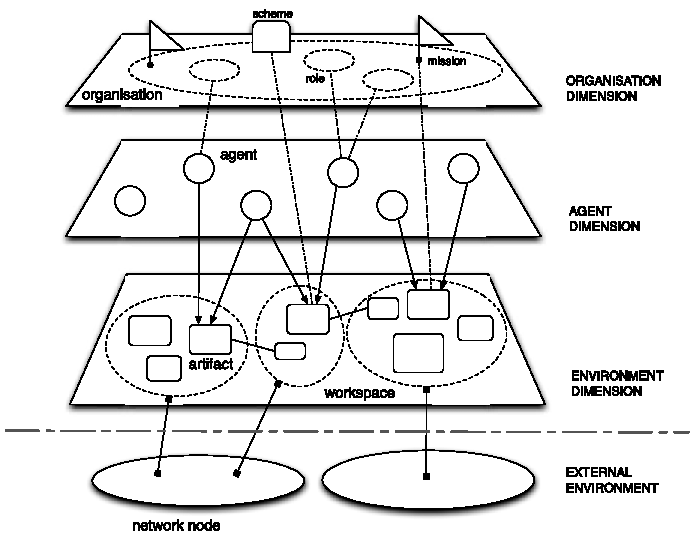
\includegraphics[width=0.9\textwidth]{figures/mas-dimensions-overview.pdf}
    \caption{High-level overview of the main programming dimensions of a \ac{MAS}, the \emph{interaction} dimension, not shown, focuses on interaction between agents, from \cite{Boissier_Bordini_Hübner_Ricci_Santi_2013}.}
    \label{fig:mas-dimensions-overview}
\end{figure}


The environment programming dimension has been introduced to recognize the environment as a first-class abstraction in \ac{MAS} programming~\cite{Weyns_Omicini_Odell_2007}.
%
In this perspective, the environment is not just a passive context, but an active component that can influence and be influenced by agents.
%
Namely, the environment can serve three major roles in supporting the activity of a \ac{MAS} at different levels: 
\begin{itemize}
    \item at a \emph{Basic Level} the environment provides access to the deployment context of the agent, allowing it to interact with external resources either them being physical (e.g., sensors, actuators) or virtual (e.g., databases, web services);
    \item at an \emph{Abstraction Level}, the environment provides a higher-level representation of the context in which agents operate bridging the gap between the low-level details and the agents' behavior;
    \item at a \emph{Interaction-mediation Level}, the environment facilitates the communication and coordination between agents, regulating access to shared resources and hence becoming an active entity in the \ac{MAS}.
\end{itemize}


Elaborating on this perspective, the \emph{Agents and Artifacts (A\&A)} metamodel, proposes to model the environment as a collection of \emph{artifacts} shared amongst agents~\cite{Omicini_Ricci_Viroli_2008}.
%
Artifacts are defined as computational entities that encapsulate both state and behavior, providing a means for agents to interact with the environment in a structured way.
%
This approach allows for a more flexible and dynamic modeling of the environment, introducing a further \emph{reflection level} where artifacts can be created, modified, and destroyed at runtime by the agent themselves, reflecting the changing needs and goals of the agents~\cite{Ricci_Omicini_Viroli_Gardelli_Oliva_2007}.

The organization programming dimension~\cite{Boissier_Hübner_Sichman_2007} focuses on the structure and roles of agent societies within a \ac{MAS}. 
%
\ac{MAS} organizations shift the focus from individual agents to the collective behavior of groups of agents~\cite{Ferber_Gutknecht_Michel_2004}.
%
Organization programming targets those kinds of \ac{MAS} where the strcture and roles within an organization are explicitly defined and managed in a top-down fashion, as opposed to emergent organizations where the structure arises from the interactions of individual agents in a bottom-up fashion~\cite{Boissier_Hübner_Sichman_2007}.

\begin{figure}[t]
    \centering
    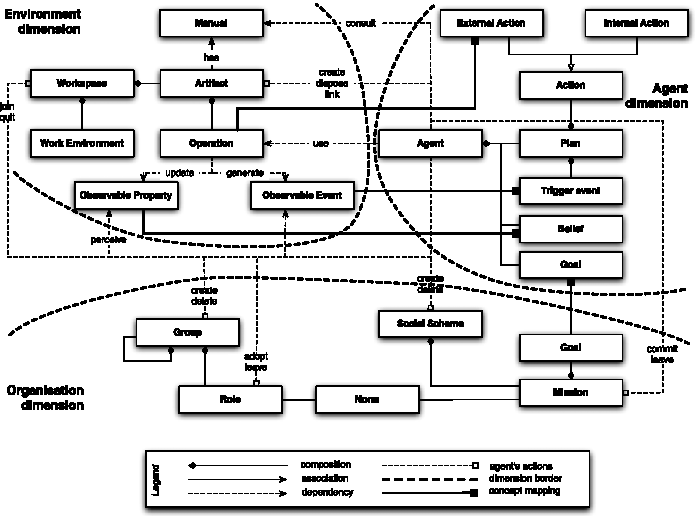
\includegraphics[width=\textwidth]{figures/mas-dimensions-schema.pdf}
    \caption{Schematic representation of the main abstractions of \ac{MAOP} and their relationships, from \cite{Boissier_Bordini_Hübner_Ricci_Santi_2013}.}
    \label{fig:mas-dimensions-schema}
\end{figure}

The proposal of \ac{MAOP} evolves \ac{AOP} to consider all the different dimensions of \ac{MAS} programming in a unified framework~\cite{Boissier_Bordini_Hübner_Ricci_Santi_2013,Boissier_Bordini_Hubner_Ricci_2020}.
%
The paradigm has been supported by the development of the \jacamo{}~\cite{Boissier_Bordini_Hubner_Ricci_2020} framework which integrates three main components:
\begin{itemize}
    \item \textbf{\jason{}}: a Java-based interpreter of \agentspeak{}~\cite{raoagentspeak} for programming and executing \ac{BDI} agents~\cite{Bordini_Hübner_Wooldridge_2007};
    \item \textbf{\cartago{}}: a framework to model and implement the environment as a set of artifacts that agents can use to perceive and act upon the environment~\cite{Ricci_Piunti_Viroli_Omicini_2009};
    \item \textbf{\moise{}}: a framework to define and manage the organization of agents in terms of roles, groups, and missions~\cite{Boissier_Hübner_Sichman_2007}.
\end{itemize}

\ac{MAOP} and the \jacamo{} framework have been widely influential in the \ac{AOSE} community, providing an integrated foundation for the engineering of complex \acp{MAS}~\cite{Boissier_Bordini_Hubner_Ricci_2020}.
%
\Cref{fig:mas-dimensions-schema} provides a representation of how the different programming dimensions of a \ac{MAS} are integrated in the \ac{MAOP} paradigm, showing the main abstractions and their interrelations.

In this thesis, when we discuss the engineering of \ac{MAS} we follow a \ac{MAOP}-inspired approach, focusing on the agent and the environment dimensions (and the A\&A metamodel in particular), as they are the most relevant for the integration of \acp{MAS} with \ac{DT}-based systems.
%
Although the organization dimension is also relevant, we do not specifically address it in this thesis, as we focus on relatively small-scale \acp{MAS} where the organization is implicit.

%=======================================================
\section{\acl{BDI} Agents}
%=======================================================
The \ac{BDI} model originated from the philosophical theory of human practical reasoning developed by Michael Bratman~\cite{Bratman1987-BRAIPA}.
%
The theory focused on the notion of \emph{intention} (i.e., the commitment to carrying out a plan of action), to describe future-directed decision-making, explaining how humans decide what to do
when they have multiple desires and goals to achieve.

The model greatly influenced the development of computational agents, 
leading to agent architectures such as the \ac{PRS}~\cite{Georgeff_Lansky_1986},
which provides a framework for implementing \ac{BDI} agents in software systems.
%
Computational \ac{BDI} agents are characterized by the following main abstractions:
%
\begin{description}
    \item[Beliefs:] a set of facts and rules representing an agent's memory, collecting knowledge about its perception of the world, itself, and other agents;

    \item[Desires:] a set of goals, representing (possibly partial) descriptions of desirable states of the world
    the agent is willing to achieve, test, or maintain;

    \item[Intentions:] a set of tasks the agent is currently committed to, in order to satisfy some of its desires;

    \item[Plans:] a set of \emph{recipes} representing the agent's procedural memory,
    hence encoding the know-how about achieving a given intention under certain conditions.
\end{description}


\begin{figure}[t]
    \centering
    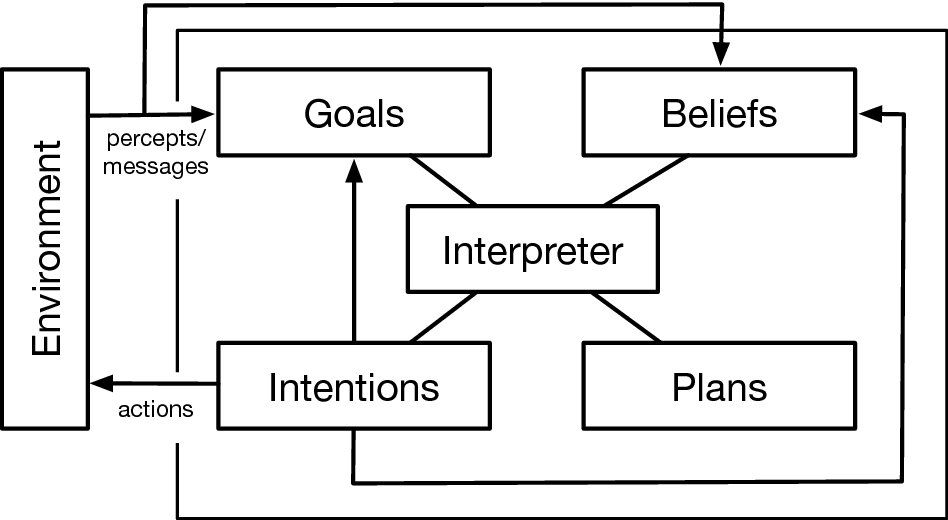
\includegraphics[width=0.9\textwidth]{figures/bdi-agent-schema.png}
    \caption{Schematic, high-level representation of a \ac{BDI} agent, from \cite{Bordini_El_Fallah_Seghrouchni_Hindriks_Logan_Ricci_2020}.}
    \label{fig:bdi-model}
\end{figure}


\Cref{fig:bdi-model} shows how these abstractions relate to each other in a schematic representation of a \ac{BDI} agent.
%
The agent acquires percepts and receives messages from other agents through the environment. This can lead to an update of the agent's beliefs or goals.
%
Based on its beliefs and goals, the agent deliberates on intentions to commit to, and selects plans to achieve them. 
%
Finally, pursuing an intention, through the execution of the selected plans may lead to actions that affect the environment. 
%
In the figure, a central \emph{interpreter} of the agent program is shown. 
%
This component is responsible for managing the agent's execution, often referred to as the \emph{reasoning cycle} of the agent.

\ac{BDI} agents continuously cycle through a reasoning process which involves three main phases:
\begin{enumerate}
    \item \emph{Perception:} the agent perceives its environment through its sensors, updating its beliefs accordingly;

    \item \emph{Deliberation:} the agent deliberates on its desires and intentions,
    possibly revising them in light of the updated beliefs;

    \item \emph{Action:} the agent selects and executes one or more plans to carry on its current intentions,
    possibly affecting the environment through its actuators.
\end{enumerate}

Through this mechanism, agents continuously adapt their behavior to the changing environment, acquire new beliefs that may influence their future behavior, and pursue their goals by executing plans.

Programming a \ac{BDI} agent involves defining its initial beliefs, goals, and a set of plans that support the agent in achieving its goals under different conditions. 
%
The \ac{BDI} model has been initially formalized with a logical language, \agentspeak{}~\cite{raoagentspeak} which later has inspired several agent programming languages. 
%
Amongst them \jason{}~\cite{Bordini_Hübner_Wooldridge_2007} is a Java-based interpreter for an extended version of \agentspeak{}, keeping the original syntax and semantics.

Custom \ac{BDI} agent programming languages, support developers in implementing \ac{BDI} agents by providing high-level abstractions and constructs that facilitate the definition of beliefs, goals and plans. 
%
This has the benefit of allowing developers to focus on the agent's behavior, rather than low-level implementation details. 

\note{reference other languages}

\note{explain why we consider agentspeak and jason here}

\note{description of agentspeak}

\todo{code examples??}

%=======================================================
\section{Web-based and Hypermedia \acs{MAS}}
%=======================================================

\note{Yggdrasil}

%=======================================================
\section{\aclp{MAS} and \aclp{DT}}
%=======================================================

\todo{integrate this}

\note{Add direct reference to Mariani et al}


AAs and DTs are not only used separately 
to deliver intelligent functionalities 
in a mutually exclusive way, 
or as alternative solutions to overlapping requirements.
Their synergistic usage is already seen in the available literature, 
especially in industrial deployments. Here, we briefly report recent surveys that highlight the rich intersection of these research areas.

The contamination of AAs in DTs is mostly related to the need to adopt a variety of artificial intelligence techniques in IoT applications, both to enhance the modelling capabilities of complex assets and to implement automatic controls.
Minerva et al.\ present a classification of DTs in relation to the level of intelligent behaviour the DT exhibits~\cite{Minerva2023}.
They identify the ultimate level of intelligent DT as a proactive (or autonomic) DT, capable of enacting autonomous behaviour based on the physical counterpart's current or future context.
This has a clear link with AAs, that are primarily used to model and encapsulate autonomous and intelligent behaviour in software systems.

Authors of \cite{Pretel2024} deliver a systematic literature review considering both MAS to create DTs and MAS to exploit DTs. 
Table 2 therein highlights how manufacturing is the main use case for synergistic AAs and DTs usage. 
This suggests that Industry 4.0 enabled by IoT technologies is a driving force for AAs and DTs applications. 
Furthermore, Table 3 therein emphasises that 73\% of the surveyed papers do not disclose the AAs and DTs development framework 
and that almost 8\% propose their own 
    (second largest percentage behind a ``team'' of 4 agent-oriented development frameworks). 
This suggests a great fragmentation of uncoordinated proposals, 
generating ``reinvention of the wheel'', especially with respect to the integration of AAs and DTs.

The survey in \cite{10.1115/1.4050244}, instead, has its main focus on DTs considering whether and how AAs (especially MAS) are used to complement the functionalities of DTs. 
Of particular relevance for the present article is Figure 5 therein, 
which reports the vision of an ``Intelligent Product'' (IP) from the literature. 
Such IP fosters the synergistic usage of DTs and AAs. 
DTs help create an ``intelligent being'', 
whereas AAs augment it with an ``intelligent agent'' to make it an IP. 
The ARTI reference architecture is inspired by these concepts, 
and it has been among the first architectures proposed to consider 
the combined usage of AAs and DTs (and the most widely adopted). 
Finally, it is relevant that also here manufacturing and IoT emerge as the main application domains for the integrated usage of AAs and DTs.

The last survey we mention is \cite{Kalyani2025}, 
where the focus is on a one-way integration of AAs and DTs: 
AAs supporting DTs implementation. 
A practical example of such an integration is given in \cite{Latsou2021811}, 
where AAs are used to create a complex DT endowed with ``intelligent'' functionalities (e.g.\ prediction). 
An interesting takeaway that the authors of \cite{Kalyani2025} get from the surveyed literature 
is that a main driving force behind this specific integration is exactly endowment of DTs with AA properties. 
In Section~\ref{sec:abstractions-and-principles} we will see how this need is captured by our principles and proposed micro-architectures for AAs and DTs integration.

Providing the complete overview 
of all the available AAs and DTs-based architectures for IoT scenarios 
is out of the scope of this paper---the interested reader is referred to these surveys. 
However, it may be beneficial for the reader
to report some selected examples.
In \cite{Nie2022}, for instance, 
    an AA is used to aggregate information from different DTs in a manufacturing scenario, 
    to predict faults in machinery and (re-)optimise production scheduling.
Another example in manufacturing is in \cite{Xu2024}. 
    There DTs are used mainly as an abstraction layer over the whole manufacturing system, 
    providing a uniform access layer to AAs. 
    AAs are used mainly to support automatic feedback control (digital to physical) 
    and communication and coordination between robot AAs, task AAs, and workstation AAs.
In \cite{DBLP:conf/pads/ClemenALOOSG21}, instead, 
    AAs are used to build the complex DT of a whole city.

It is also worth noting that there may be literature, such as reference \cite{DBLP:journals/jiii/BiZWL22}, 
where the term ``autonomous agent'' does not appear, 
but whose proposal is well aligned with the literature about AAs. 
For instance, in the mentioned paper, 
a Digital Triad is proposed as an advancement beyond DTs, 
where design knowledge and application-specific intelligence is encapsulated 
in a very similar way to AAs. 
Surveying all of this ``submerged'' literature is a complex task given that terminology likely do not match. 
However, we hope that our contribution can promote cross-fertilisation with these related research efforts, 
in a joint effort to avoid reinventing the wheel---our main motivation for sticking to AAs instead of introducing brand new concepts into DTs.
    
%======================================================
\subsection{Intelligent functionalities for AAs and DTs}
\label{ssec:functions}
%======================================================

The literature on distributing intelligence in IoT discussed in previous sections reports on several intelligent functionalities for which AA and DTs are being actively used by system designers. 
%
We summarise and categorise them here regardless of the specific task they accomplish (e.g.\ time series forecasting vs.\ fault prediction) and of the specific technique adopted (e.g.\ regression, SVM, etc.), but focussing on the \textit{kind} of intelligent function they deliver.
%
This categorisation is useful first of all in defining what we can consider, for the scope of this paper, ``intelligence'' in a practical, bottom-up way, stemming from related works in the area without getting trapped in philosophical arguments. 
%
Then, it is also useful to establish the \emph{coverage} of such functionalities by AAs and DTs, as shown in Figure~\ref{fig:radar-aa-dt}, which already suggests that they can be used synergistically to deliver the full spectrum of such intelligence. 
%
\begin{itemize}
    \item \emph{Prediction}, there including time series forecasting, recommendations, namely any form of reasoning meant to ``guess'' new information based on past and current knowledge. 
    In the IoT, common prediction targets are machinery failures, stock levels, resource use, and system states. 
    \item \emph{Simulation}, encompassing any form of reasoning by hypothesising different states, in the past, present, or future. 
    ``What-if''-like analysis falls into this category. 
    In the IoT, it is common to simulate the future states of individual things, for example, to improve the design of a product or a production pipeline. 
    However, complete systems can also be simulated with an added degree of complexity.%usually integrate multiple AAs and DTs in hierarchical architectures. 
    \item \emph{Planning}, that includes any form of synthesis, and \emph{practical reasoning}~\cite{Bratman1988}, which is meant to figure out how to achieve some practical effect (on the target system) by properly sequencing available actions. 
    Planning to achieve a given system configuration is common in the IoT, as well as planning to reconfigure after some disruptions. 
    \item \emph{Inference}, within which we include both \emph{epistemic reasoning}~\cite{Meyer1995}, that is, synthesising novel information from known data, or data-driven inference such as pattern recognition and classification.
    This is perhaps the most common form of intelligence used in IoT, as even simple monitoring and control applications usually infer situations by aggregating different data coming from distributed sources of information. 
    In addition, fault detection and diagnosis can be gathered in this category. 
    %    \item \emph{Diagnosis} \ste{Tutti}{a pensarci bene è una forma di inference imho, che dite?} \samu{Ste}{La definizione di inference è veramente larga quindi ci cade dentro quasi tutto sì.. io ci ho fatto ricadere anche detection poi nella 4}
    \item \emph{Adaptation} instead gathers all the intelligent functionalities aimed at enabling the system to adapt to unforeseen situations that had not been explicitly managed at design time. 
    As in the previous category, this one is quite broad and includes several heterogeneous approaches, ranging from engineered adaptation (e.g.\ the MAPE-K loop~\cite{Oh2022}) to learning-based methods (e.g.\ evolutionary approaches~\cite{Eiben2005}). 
    \item Finally, we highlight the role of \emph{Learning}, which despite not usually being the primary goal for a functionality, is a valuable tool to implement some of the ones highlighted above and still poses important requirements on the architecture of a system that wishes to support any form of learning process in one of its components.
    That includes statistical machine learning, reinforcement learning, and causal structure learning~\cite{Bordini2020-AI,Erduran2023,Mariani2023a,Mariani2023}. 
    In this category, we group the functionalities that aim to make the system, or one of its components, learn to do something. 
    In IoT, the most common form of learning employs statistical machine learning to create prediction models, for example. 
\end{itemize}
%
The next Section refers to these categories of intelligent functionalities to illustrate why and how to use the design principles proposed therein.



%=======================================================
\section{Final Remarks}
%=======================================================